\documentclass[report]{iisthesis}
%           or master (bachelor or master is required)

% These two packages are highly recommended:
\usepackage[T1]{fontenc} % make non-ASCII characters cut&pastable in PDF
\usepackage{lmodern}     % easiest way to get outline fonts with T1 encoding
\usepackage{subcaption}
\usepackage{amsmath}


% \usepackage[ngerman]{babel}     % if the thesis is written in German

\title{Rotating Table Task with Reconfigurable Behavior Trees}
\author{Fabian Amhof \\ Matteo Quaratino}
\supervisor{Dr. Matteo Saveriano}
%\supervisor{Firstname1 Lastname1\\ Firstname2 Lastname2}

\begin{document}
\maketitle
\pagenumbering{arabic}
\chapter{Abstract}
In this project we have a rotating table with an object on it. The task is to grab this object with a "Franka Emika Panda Robot", pick it up, and then place it again on the table. 
Some work was provided from last years course, where the basic functionality is already implemented. 
The robot already grabs the object and places it again on the table but in a way that can be improved in many terms.
This implementation does not estimate the table velocity, a static offset to the objects position was hardcoded. This resulted in the robot pushing the cube off the table in some situations.\\
We will use a framework for RBTs to implement a customizable implementation of the given project allowing for improved reusability of the code. 

\tableofcontents
\label{chap:declare}

\chapter{Improvements}
\label{improvements}

\section{Control Robot by ROS-node on external machine}
\label{separate_node}
We propose to control the robot with a ROS-node on a external machine. 
We think that it is more flexible, so you can easily change the ROS-node to reconfigure the robots behaviour without changing the scripts on the robot itself. In addition to that an external node allows we can write full-fledged software and not just
some scripts, expecially in regard to the RBT it's beneficial

\section{Estimate Table Velocity}
\label{estimate_velocity}
In the example we were given the robot arm does not adjust its movement in relation to the speed at which the table 
turns. The timing and movement speed is hardcoded, and so is the speed of the table. \\
We want to work on this by letting the arm adjust its movement dynamically to the table speed.

\section{Improve Grabbing Capabillities}
\label{improve_grabbing}
The grabbing motion of the current implementation is reliant on the table turn speed being a specific and constant value, since it's hardcoded. If it varies even by the slightest bit
the arm could potenionally run into problems and for example push the cube off the table, ideally this should not happen at all. \\
We want it to react accordingly by building on \ref{estimate_velocity}, assuming that a faster cube is harder to grasp, it might be necessary to define another grabbing motion 
or at least change it for different situations, like a uneven speed of the table. \\
In the given implementation the gripper does not rotate according to the alignment of the cube. The robot is not using joint number 7, which is responsible for the rotation of the gripper, we would like to try to allow the arm to adjust the angle of the gripper accordingly.
If all goes well, a option to reposition a misaligned cube could also be implemented.

\section{Implement RBT}
\label{implement_rbt}
That highlevel desicion making, for example if the robot should move its arm or try to grab something, can be done with behaviour trees or reconfigurable behaviour trees.
Reconfigurable behaviour trees are an extention of standard behaviour trees and provide a more dynamic and resource-saving approach to represent a task.
We will use RBT to plan the actions the robot should make in order to execute the task successfully. RBTs can execute different BT based on the priority of each subtask. The priority gets influenced by sensory data or states.
Based on the following parameters we would like to change priority of the different subtasks. Each subtask is represented in its own BT.
\begin{center}
    \begin{tabular}{ |c|c||c|  }
        \hline
        Object in reach & Object grabbed & Priorized Task \\
        \hline
        \hline
        False & False & Wait \\
        False & True & *Not possible* \\
        True & False & Grab Object \\ 
        True & True & Place Object on Table \\
        \hline
    \end{tabular}
\end{center}
\noindent
Since this is a relatively easy task it would be also easy to represent it with a normal BT. However when we use a RBT the table above would be a way how to deal with priorities. Another way is to just consider the distance of the object in the priority function and use the parameter "object grabbed" as precondition for the task "Place Object on Table".
Therefore if the object is not in reach the robots executes the "wait" task and when the object is in reach the instanciator first checks if the condition "object grabbed" is set. If it is set, then "Place Object on Table" gets executed, if not then "Grab Object" gets executed.

%\section{Use Camera to detect Cube [OPTIONAL]}
%\label{use_camera}
%Another thing that could be improved is the recognition of the object. At the moment, thanks to the simulation, we know the position of the object and so we dont have to recognize it. In the real world however we need some sensor to determinate the position and orientation of the object that we need to pick up. For this one could use a camera and then, based on the position of the camera and the image check where the object lies on the table. \\
%We would like to focus on the previous points and add this feature only when we're satisfied with section \ref{separate_node} to \ref{implement_rbt}. 

\setcounter{chapter}{1}
\setcounter{section}{0}
\chapter{Starting point}
This report builds on a previous work where a 'Franka Emika Panda Robot' grabs a object from a rotating table and places it again.
The previous implementation had inverse kinematics already in place which we decided to keep. Furthermore all the code was done in LUA scripts, directly in CoppeliaSim which had to be moved to a external ROS-node to facilitate the addition of the reconfigurable behaviour tree.
Many parameters such as the time the arm takes to reach a position and the offset, that is needed to 'catch' the object in time, were hardcoded. This poses a problem when the speed of the rotating table changes and will be calculated dynamically in our implementation.\\
We were provided with the framework for the 

\begin{figure}[h]
    \caption{Franka Robot in CoppeliaSim}
    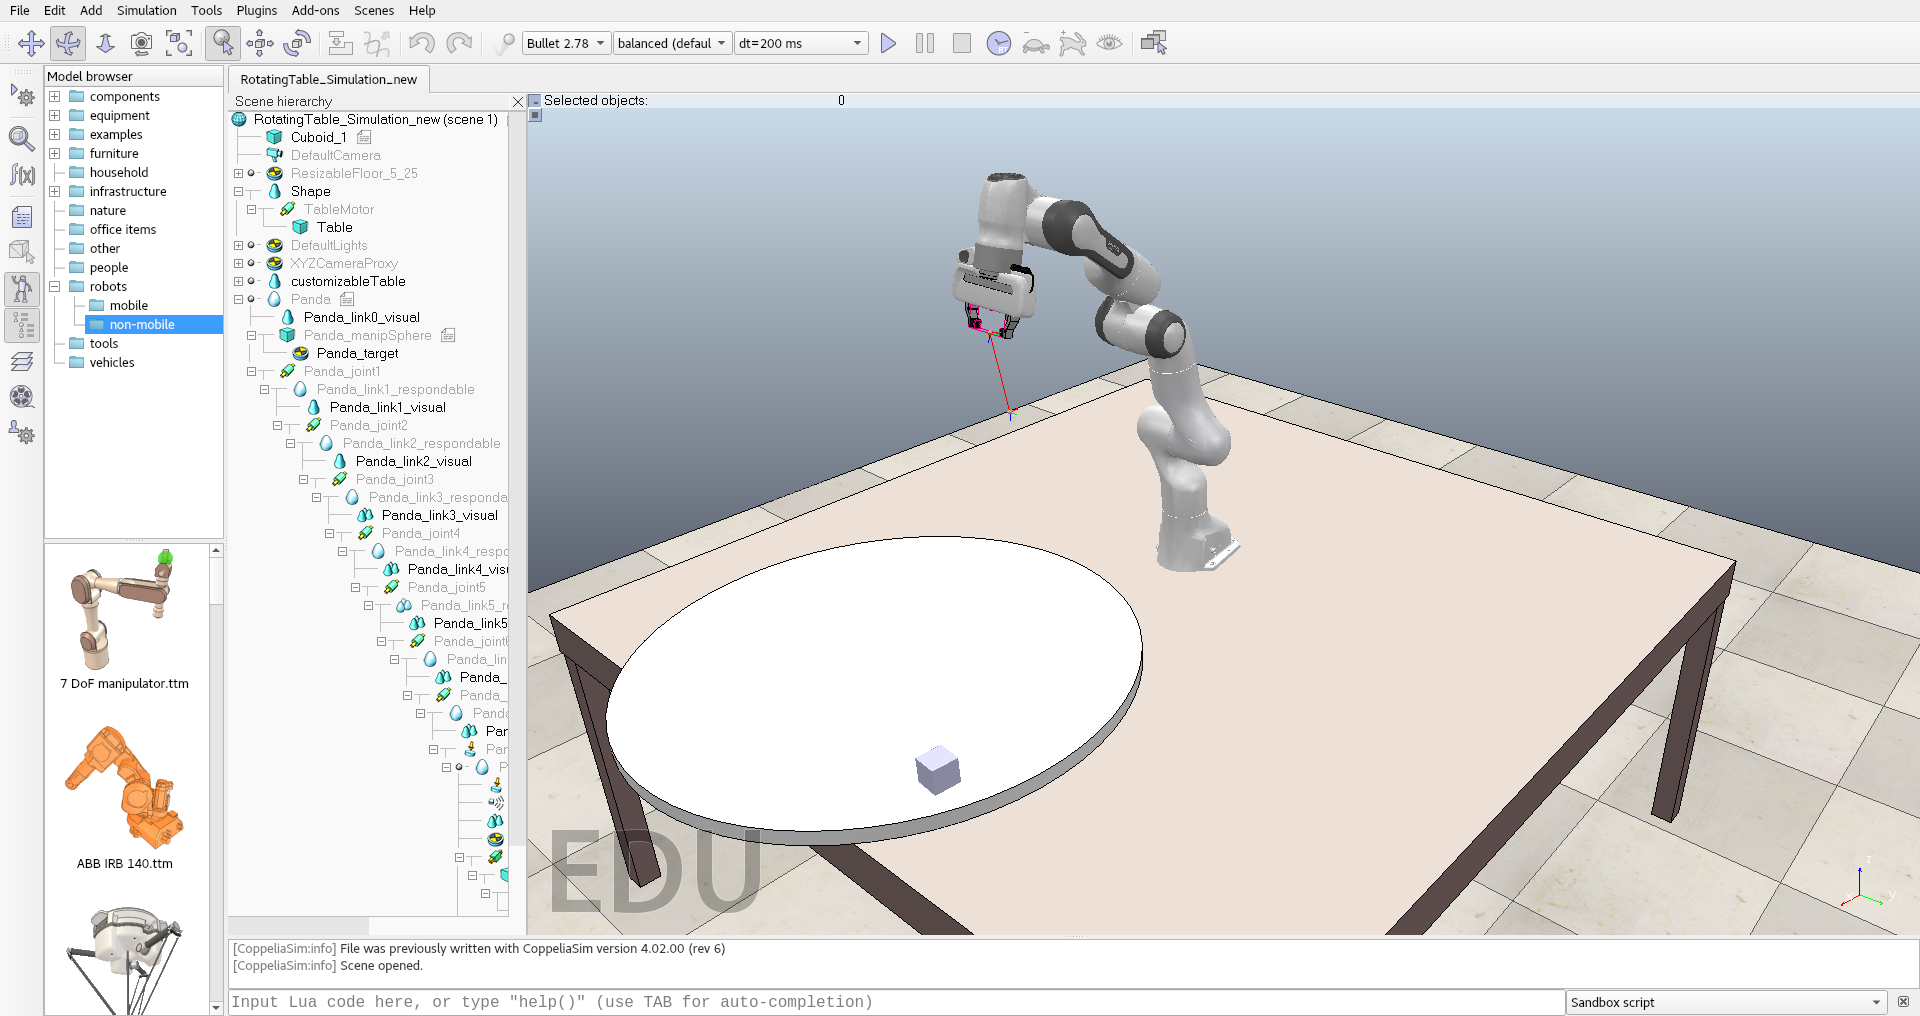
\includegraphics[width=\textwidth]{arm_coppeliaSim}
\end{figure}
\noindent
The RBT framework provided to us requires Python 3.8 and the programm could misbehave if not run correctly.
A guide on how to execute the code of this project can be found in the readme of the github repository. 

\setcounter{chapter}{2}
\setcounter{section}{0}
\chapter{Implementations}
Here we document the realisazion of the suggested improvements.

\section{External ROS-node}
The first thing that had to be done was to allow the robot to interface with a python program.
This was important since the code for reconfigurable behaviour trees was implemented in python, so it would be easiest way to control the 
arm.
We created a few ROS-topics that would be useful:

\begin{description}
    \item [cube\_ori] the orientation of the cube in euler coordinates 
    \item [cube\_pos] the position of the cube in relation to the robot arm
    \item [gripper\_pos] controls (open, close) of the gripper
    \item [gripper\_state] returns if the gripper has grabbed a object or not
    \item [robot\_state] integer which determines the state in which the robot is 
    \item [target\_pos] the position to which the gripper will move
\end{description}
\noindent
Firstly we moved the whole control of the arm from the LUA-script to a external python program, keeping only the inverse kinematics.
After this we could start to work on our suggested improvements. 

\section{Reconfigurable Behavior Trees}
Next the RBT \cite{DBLP:journals/corr/abs-2007-10663}, which was written in python was added. \\
This allowes to create trees in .json, which control the the arm, instead of using the automata-like system
from before.
Building on the code given to us we can program the necessary steps which will then be used by the tree when controlling the arm, e.g. prediction of
the future position of the cube and its orientation. \\
The advantage of behaviour trees is the reusability of code the main drawback here is the problmatic integration of control features. \cite{DBLP:journals/corr/abs-2007-10663}
This is because control features cannot be read instantly.
RBT address this issue by implementing parallel nodes witch allow for consistent calls on the our features. \\
In the following subsections each tree used by the robot will be briefly described:

\subsection{Basic tree}
This tree is the one used to to call the remaining individual trees to perform the grabbing task. Firstly it inizializes the blackboard, which in the RBT framework we were provided
is a container for variables which can be used by multiple nodes to exchange data. The blackboard is also useful when working with ROS-topics, allowing to just put them in a .json file and subscribing them automatically with a python programm.
Lastly the priorities are handled with the accordongly named node and a tree for each situation is chosen and switched to.
The handle Pryority action determines which tree should be executed at any time. That specific subtree is then called each time a change in priority was detected. 

\subsection{Init tree}
The init tree is called only once and is used to firstly move the arm into a standard position and than perform a calibration movement, in order to get a approximate movement speed. 

\subsection{Wait tree}
The wait tree is self explainatory, it waits until the object on the table is in reach of the arm.
Specifically it opens the gripper and moves to a neutral position.

\subsection{Pickup tree}
The pickup tree manages the grabbing of the cube and is called when the object on the table is in reach of the arm. \\
The first thing it does is check if the arm is ready and opens the gripper. Then a intermediate position is calculated using the tables rotational speed, this means that the arm will move to a predicted point above the cube and is done
so that the arm will move in on the cube from above, avoiding pushing it around or even knocking it off the table. Then again using the rotational speed of the table and the estimated travel time of the arm, a new point is calculated.
This time the gripper will move directly onto the cubes predicted position, once reached it closes the gripper and lifts the cube off the table.

\subsection{Placedown tree}
Lastly the placedown tree moves the gripper, holding the cube, back into its neutral position. Once reached the point at whitch the object should be placed is calculated and the arm moves to it.
The cube is released, and the gripper moves up before returning to the neutral position avoiding misplacement.

\begin{figure}[h]
    \centering
    \begin{subfigure}[b]{.45\linewidth}
    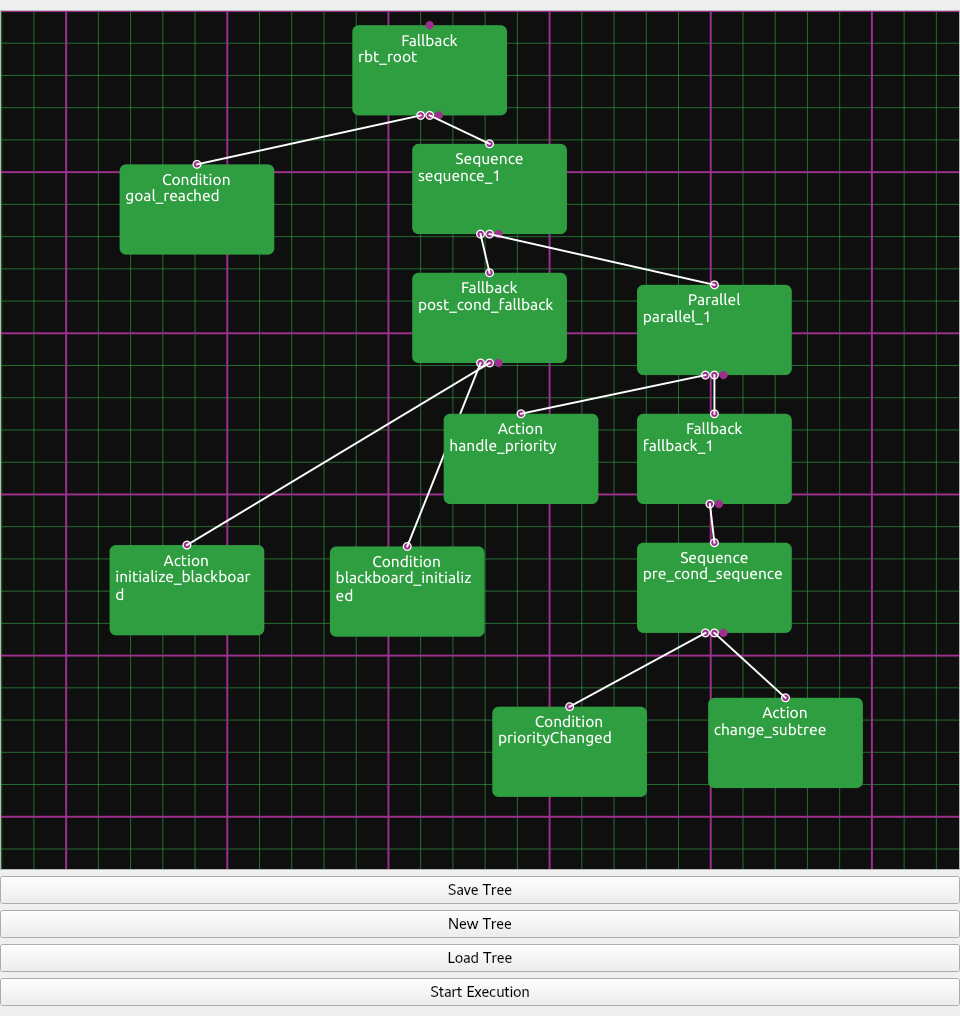
\includegraphics[width=\linewidth]{basicTree.png}
    \caption{Basic Tree}
    \end{subfigure}

    \begin{subfigure}[b]{.45\linewidth}
        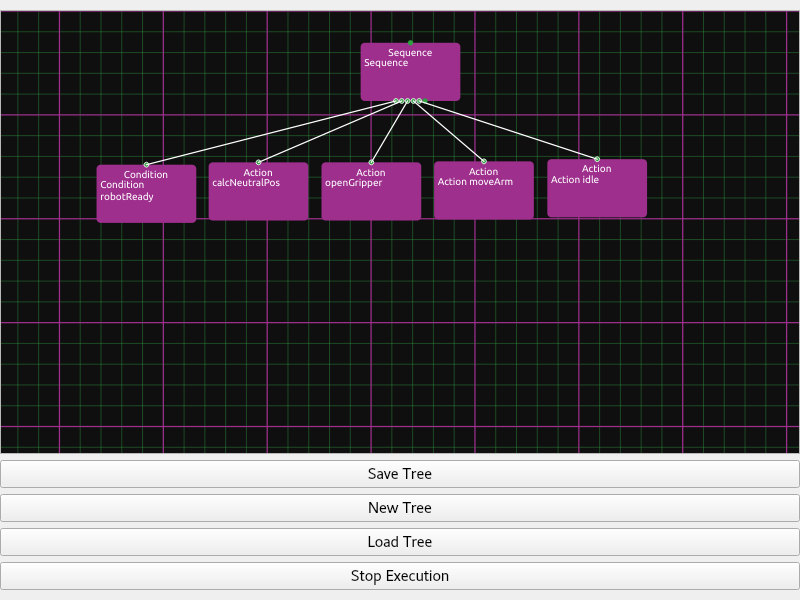
\includegraphics[width=\linewidth]{waitTree.png}
        \caption{Wait Tree}
    \end{subfigure}
    \begin{subfigure}[b]{.45\linewidth}
        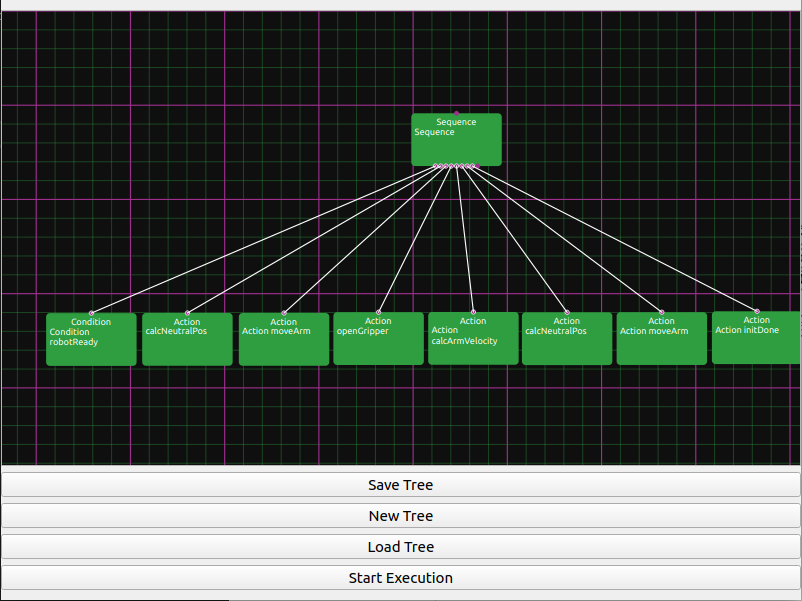
\includegraphics[width=\linewidth]{initTree.png}
        \caption{Init Tree}
    \end{subfigure}

    \begin{subfigure}[b]{.45\linewidth}
        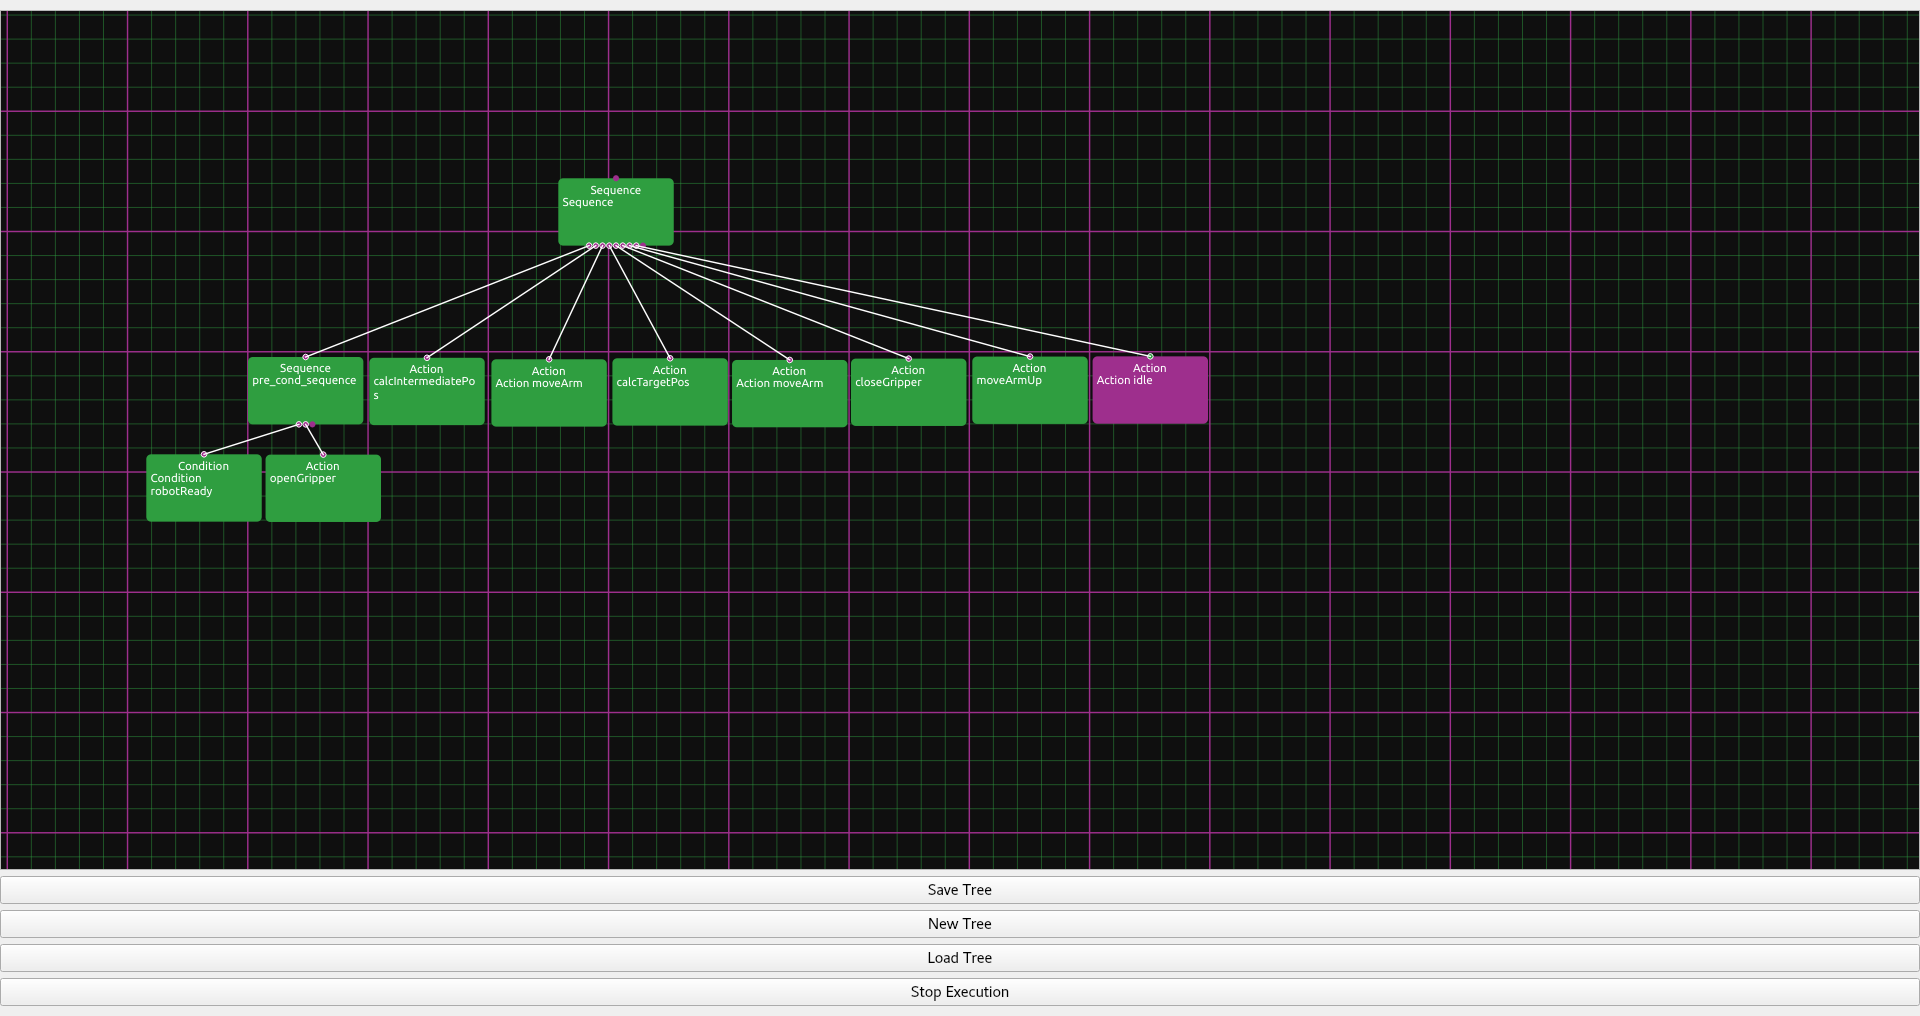
\includegraphics[width=\linewidth]{pickupTree.png}
        \caption{Pickup Tree}
    \end{subfigure}
    \begin{subfigure}[b]{.45\linewidth}
        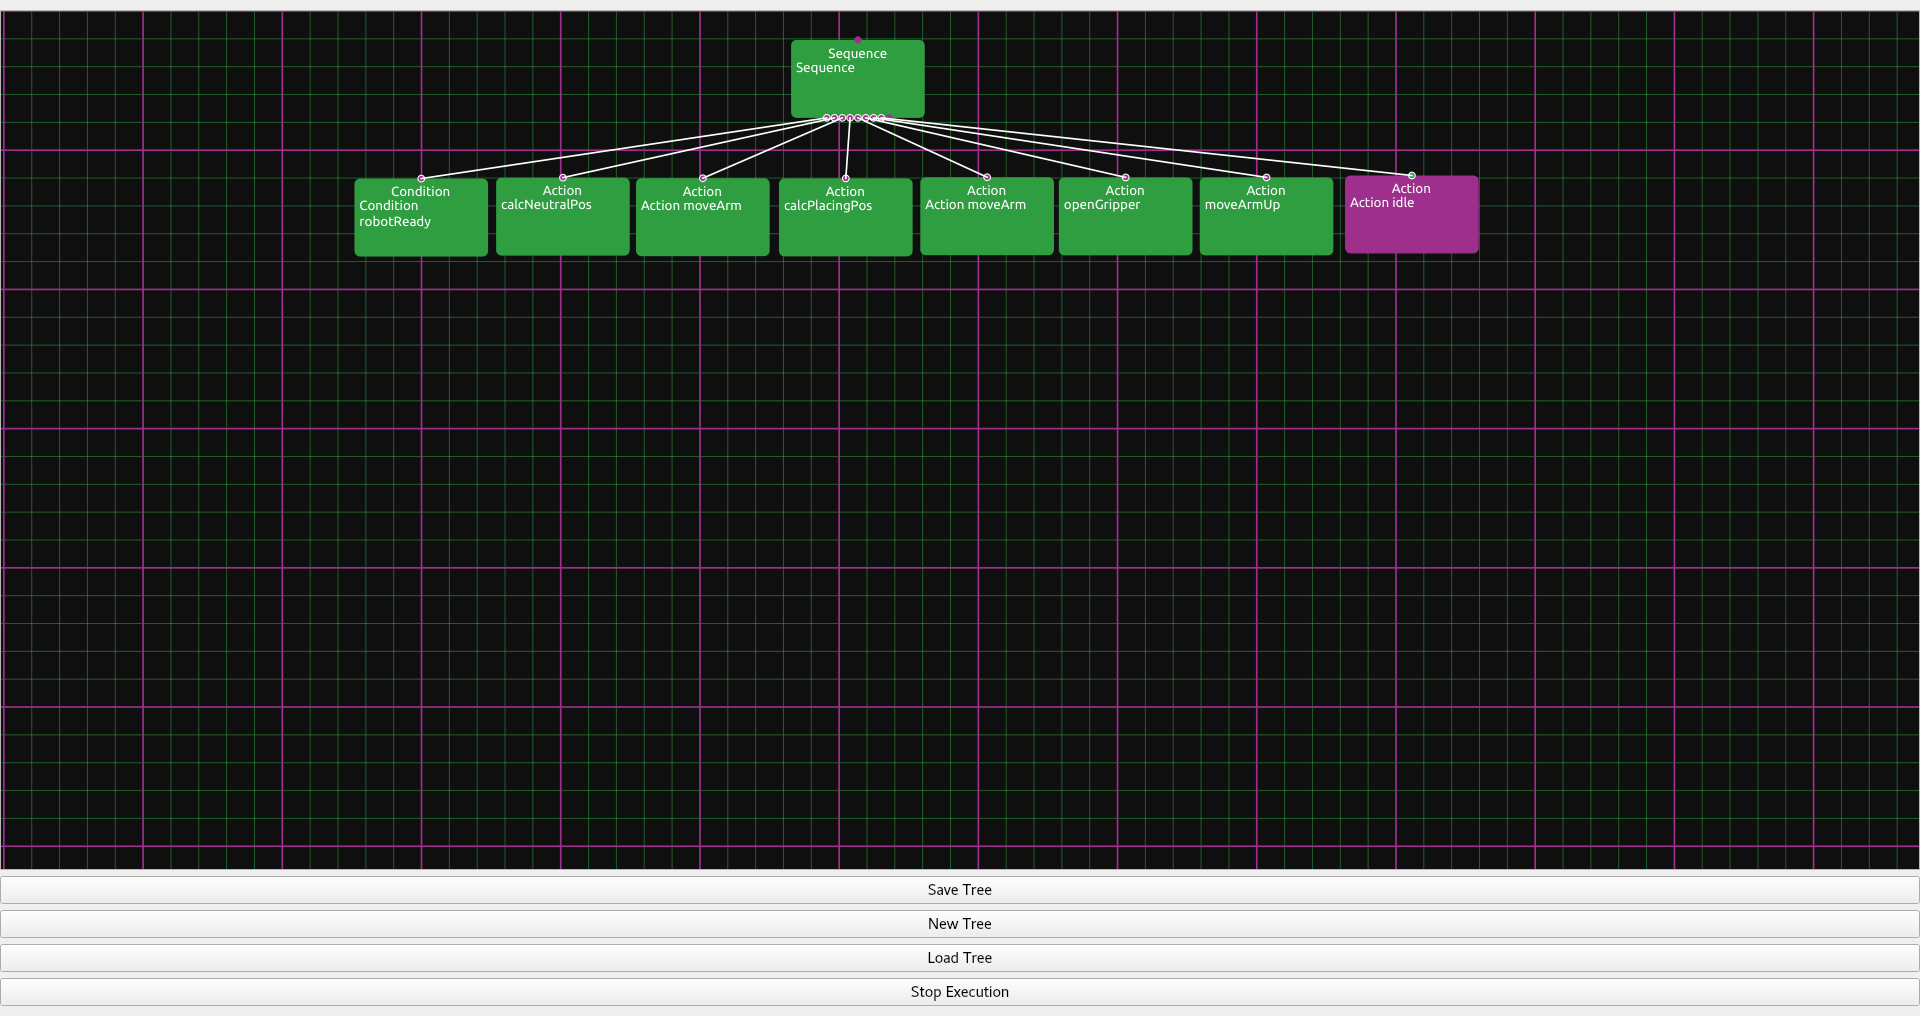
\includegraphics[width=\linewidth]{placedownTree.png}
        \caption{Placedown Tree}
    \end{subfigure}
    \caption{The trees in treeviewer.py}
\end{figure}

\section{Determine table velocity and predicted position}
By measuring the position two times with a delay inbetween, we can calculate the rotational speed of the object and predict its position after a given peiod.
This is done whith linear algebra using a third point, the tables center. The center of the table is hardcoded, to avoid using a additional topic for a value that will not change during the simulation. \\
The angle is calculated as follows:
$$
\theta = \arccos \left ( \frac{\overrightarrow{P_cP_s} \cdot \overrightarrow{P_cP_e}}{\left | \overrightarrow{P_cP_s} \right | * \left | \overrightarrow{P_cP_s} \right |} \right) \\
$$
$P_c :=$ Center of table \\
$P_s :=$ Starting point of measurement \\
$P_e :=$ Endpoint of measurement \\

In order for the predicted position to be accurate the arms movement velocity and its distance from the cube has to be estimated aswell.
The last point is quite problematic, in order predict the cubes position we need the time that the arm takes to reach that position and not knowing the position means we can't calculate the travel time, 
essentially we two unknown variables.
To circumvent this, the travel time to the cubes last known position is used instead, this means that the arm will arive at the predicted point before the cube 
and therefore the gripper will not move in a perfect vertical motion. In practice this did not impact the action but could cause problems if the shape of the object on the table was different.
Since the same argument could be brought up for a vertical movement we kept this implementation because it does not affect the cube. \\
With the angle, the delay between measurements and the arms movementspeed a position can be predicted using a simple rotational matrix:
$$
\theta_{pred} = \frac{\theta}{t_m} * t_t
$$
$t_m :=$ time between measurments \\
$t_t :=$ traveltime of arm 
$$
P_{pred} =
\begin{pmatrix}
    \cos\theta_{pred} & -\sin\theta_{pred} \\
    \sin\theta_{pred} & \cos\theta_{pred}
\end{pmatrix}
\cdot \overrightarrow{P_cP_e}
+ P_c
$$
The rotational matrix is only 2D because the calculation was done on a plane to simplify things. The z-value was set to a constant value in order to return to 3D. 

\section{Improved Grabbing Capability}
When the simulation starts the cube is aligned in a way that allows the arm to grab it correctly. If the object gets pushed or dropped on the table incorectly the grabbing action could run in to problems
on the next round. To avoid this we added the capability for the gripper to rotate and adjust itself to the cubes orientation.
The orientational coordinates are defined in euler angles and can be passed via a topic using a 3D-vector.
Euler angles are a set of 3 angles, which define the pitch roll and yaw of of a object. In this scenario the yaw is most important, since we can use it to rotate the gripper on its vertical axis.
The main problem when setting the yaw of the gripper to match the one of the cube was that axis of the robot and the ones of the cube do not start facing the same way, even if the shape of the cube allowes 
to pick it up when it is laying on the 'wrong face' it is easier to normalize its coordinates so the gripper can be controlled the same regardless which direction the cube faces. 
Should the cube be flipped for whatever reason between turns the gripper will always move in to grab it from above.
As a side benefit this means that the gripper avoids unnecessary 180° turns.

\setcounter{chapter}{3}
\setcounter{section}{0}
\chapter{Reusability, Applicability and Possible Problems}
The implementation we provide can be reused and repurposed easily since it is based on reconfigurable behaviour trees. The reconfigurable behaviour trees allow to alter the arms functionality
by adding actionnodes or expand on them. This makes it more customizable than the version which was given to us. \\
If the project was to be ported to a physical version some adjustments have to be made:
\begin{description}
    \item[Object position] The arm gets its target position from the RBT via ROS-topics, it is calculated with the cube position, which in turn is also a ROS-topic. In order for a physical arm to know where to move, a sensor or camera needs to be put in place instead. 
    \item[Grabbing different objects] The current implementation is intended for objects that can be picked up from above. In our scenario this works fine, should this implementation be used in the physical world where objects might be too delicate or the shape is impossible
    to grab from above, the gripper motion has to be reworked, this can be done on top of the existing work.
\end{description} 
\noindent
\section{Basis for future scenarios}
The current functionallity can repurposed to solve other problems with not much alteration.
\begin{itemize}
    \item The arm can handle multiple objects if orientation- and position-topics are added for ROS and the action nodes are modified to check each ones position. 
    \item If the objects were on a convejor belt calcPos.py can be changed to predict the future position on a linear trajectory instead of a rotational one.
    \item If only certain kinds of objects should be grabbed a condition can be added in handlyPriority.py. These objects can be moved from one moving table to another or sort them.
\end{itemize}


\bibliography{refs}
\end{document}
